\section{Podobné aplikácie}
\subsection{Mapbox}
Mapbox je platforma údajov o polohe pre mobilné a webové aplikácie\cite{mapbox}. Poskytuje mnoho produktov: \textit{Mapbox GL JS} knižnicu, pomocou ktorej je možné vytvoriť interaktívnu, prispôsobenú a efektívnu mapu vo webovej aplikácii\cite{mapbox_gljs}, \textit{Navigation SDK for mobiles}, riešenie pre vytváranie navigácie v mobilných telefónoch dostupné pre \textit{Android} aj \textit{iOS}\cite{mapbox_mobile_navigation},  \textit{MapGPT}, prvého \acrshort{ai} asistenta, s ktorým je možné mať konverzácie ohľadom ciest, navigačných inštrukcií alebo atrakcií\cite{mapbox_mapgpt}. Výhody Mapboxu:
\begin{itemize}
  \item Ponúka 50 tisíc načítaní mapy vo webovej aplikácii.
  \item Poskytuje map-matching, ktorý pripne vstupné GPS údaje trasy k cestnej sieti pre zaručenie prehľadného zobrazenie trás, to znamená, že trasy nebudú zobrazené mimo cesty ale budú ležať na cestnej sieti.
  \item Prispôsobenie štýlov mapy, markerov alebo vyskakovacích okien.
\end{itemize}
Nevýhody
\begin{itemize}
  \item Neposkytuje vlastnú webovú aplikáciu, na ktorú je možné nahrať trasu, ktorú chceme zobraziť. Trasa sa dá zobraziť až po použití Mapbox GL JS a implementovaní vlastnej webovej aplikácie.
  \item Vstupné dáta treba upraviť na požadovaný formát pred odoslaním do Mapbox \acrshort{api}.
  \item Do jednej požiadavky na map-match je možné vložiť len 100 bodov, preto je potrebné pre dlhšie trasy (tisíc bodov a viac) urobiť niekoľko požiadaviek. Pri aplikácií, ktorú používa veľa používateľov (rádovo tisíc) môže rýchlo dôjsť k vyčerpaniu kvóty pre map-match (100 tisíc mesačne) zadarmo. Taktiež rozdelenie trás do viacerých požiadaviek spomaľuje rýchlosť map-matchingu.
  \item Trasa je ku cestnej sieti pripnutá nepresne, viď obrázok \ref{fig:mapbox-map-match-vs-valhalla}.
  \item Je potrebné použiť online \acrshort{api}, čo môže spomaliť map-matching.
\end{itemize}
\begin{figure}[H]
  \centering
  \begin{subfigure}{.45\textwidth}
    \centering
    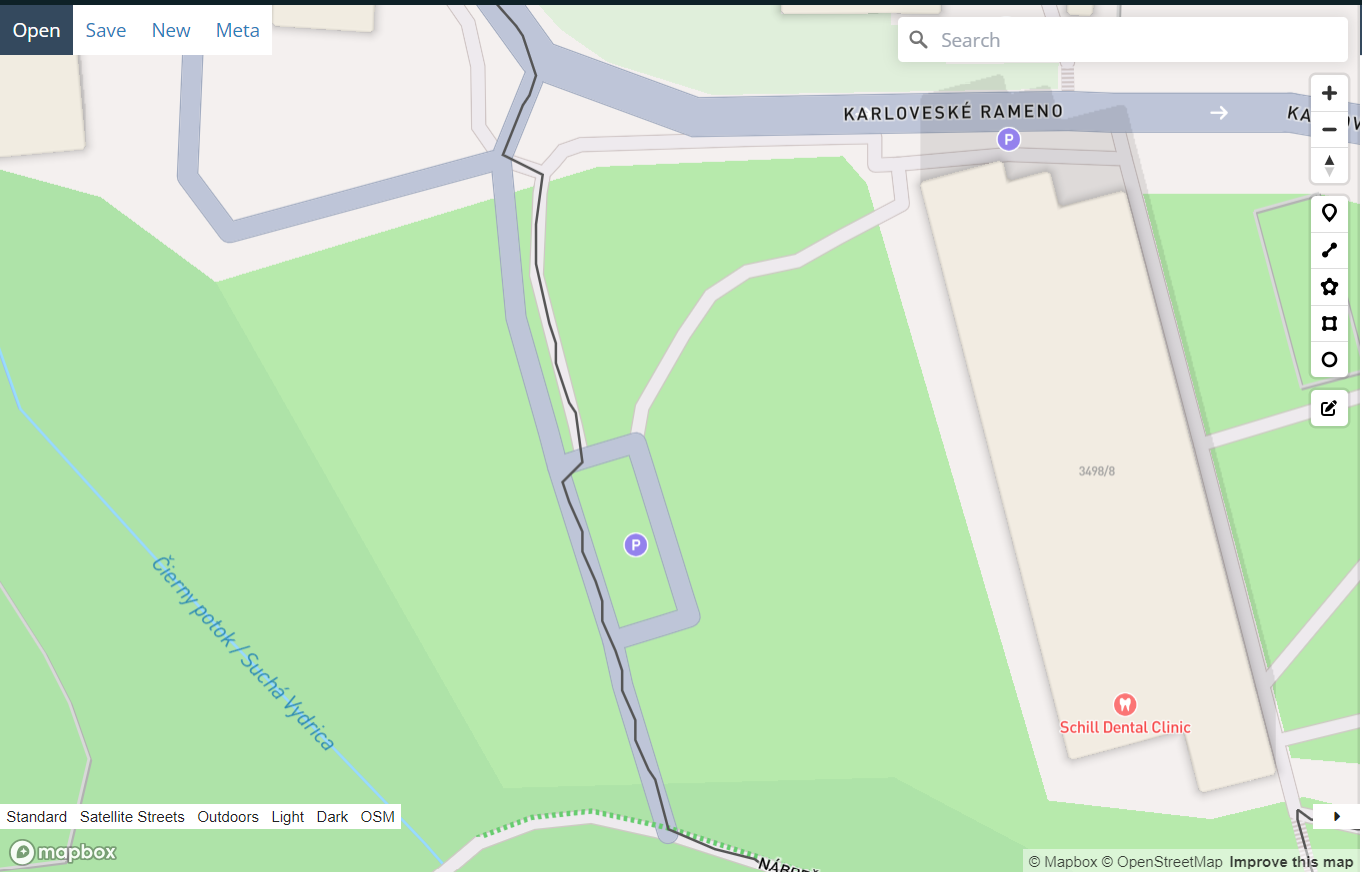
\includegraphics[width=1\textwidth]{img/porovnanie_map_match/mapbox-map-match.png}
    \caption{Map-match od Mapbox}
    \label{fig:mapbox-map-match}
  \end{subfigure}
  \begin{subfigure}{.45\textwidth}
    \centering
    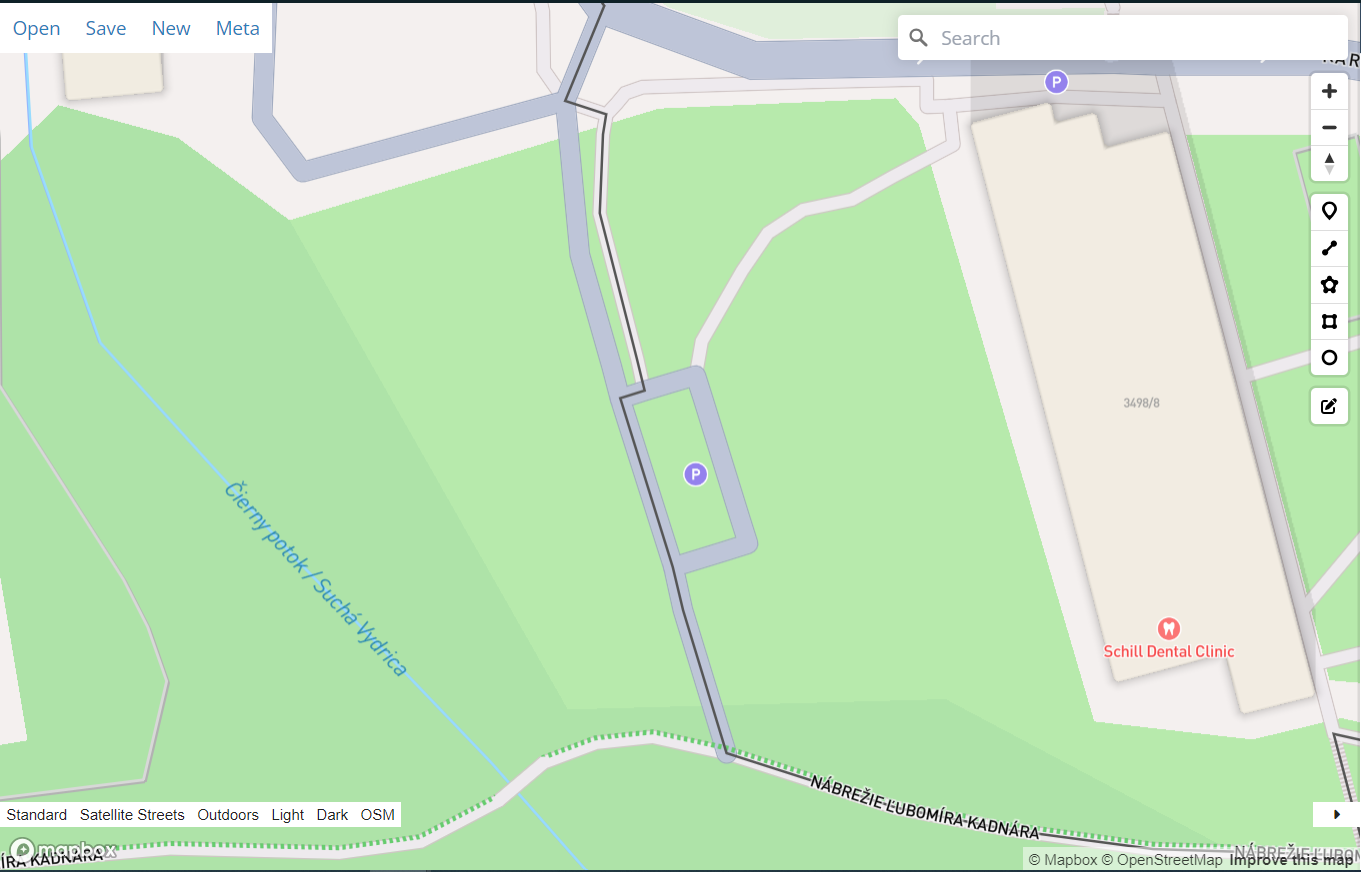
\includegraphics[width=1\textwidth]{img/porovnanie_map_match/valhalla-map-match.png}
    \caption{Map-match od Valhally}
    \label{fig:valhalla-map-match}
  \end{subfigure}
  \caption{Porovnanie Mapbox a Valhalla map-matching}
  \label{fig:mapbox-map-match-vs-valhalla}
\end{figure}

\subsection{GPS Visualizer}
GPS Visualizer je online nástroj, ktorý vytvára mapy a profily z geografických údajov. Ľahko sa používa, je prehľadný a rýchly, to znamená, že pri prvom pohľade na nástroj používateľ vie, ako nástroj používať. Vstup môže byť vo forme údajov GPS (trasy a body na ceste), jazdných trás, ulíc alebo jednoduchých súradníc. Používa sa na zobrazenie trás, plánovanie trasy alebo na rýchlu vizualizáciu geografických údajov (na vedecké pozorovania, zobrazenie nehnuteľností, geograficky označených fotografií a podobne). Na webe je od októbra 2002\cite{gps_visualizer}. Výhody:
\begin{itemize}
  \item Rýchly, prehľadný a ľahký na použitie.
  \item Dokáže načítať dáta z rôznych zdrojov (GPX, URL, FIT, CSV, TRK a ďalšie).
  \item Mapu so zobrazenou trasou je možné stiahnuť vo formáte HTML stránky na neskoršie zobrazenie.
\end{itemize}
Nevýhody:
\begin{itemize}
  \item Neponúka map-matching, iba zobrazuje trasy.
  \item Pre zobrazenie trasy je nutné zakaždým nahrať súbor s GPS údajmi.
  \item Nutnosť pripojenia na internet kvôli načítaniu knižníc.
\end{itemize}
Prostredie GPS visualizer je zobrazené na obrázkoch nižšie \ref{fig:gps-visualizer}.
\begin{figure}[H]
  \centering
  \begin{subfigure}{.7\textwidth}
    \centering
    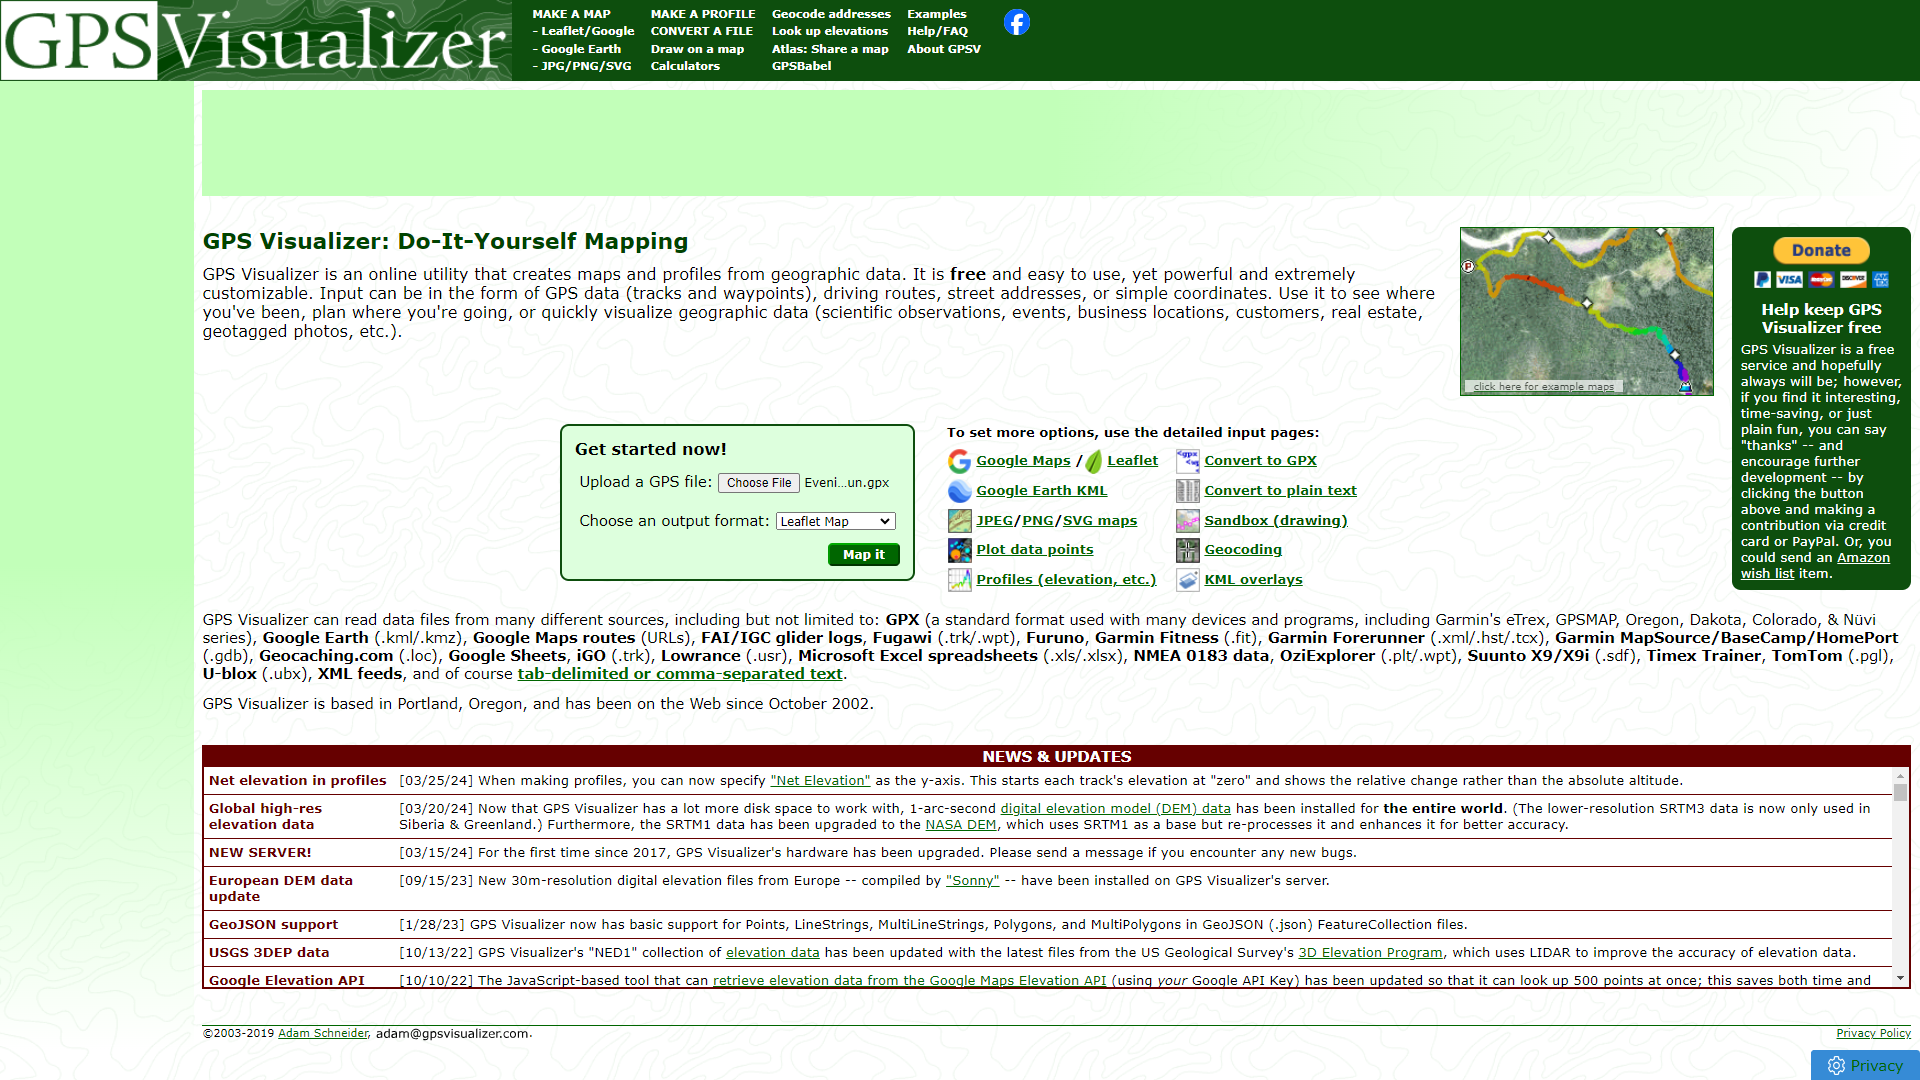
\includegraphics[width=1\textwidth]{img/gps_visualizer/gpsvisualizer1.png}
    \caption{Nahratie trasy}
  \end{subfigure}
  \begin{subfigure}{.7\textwidth}
    \centering
    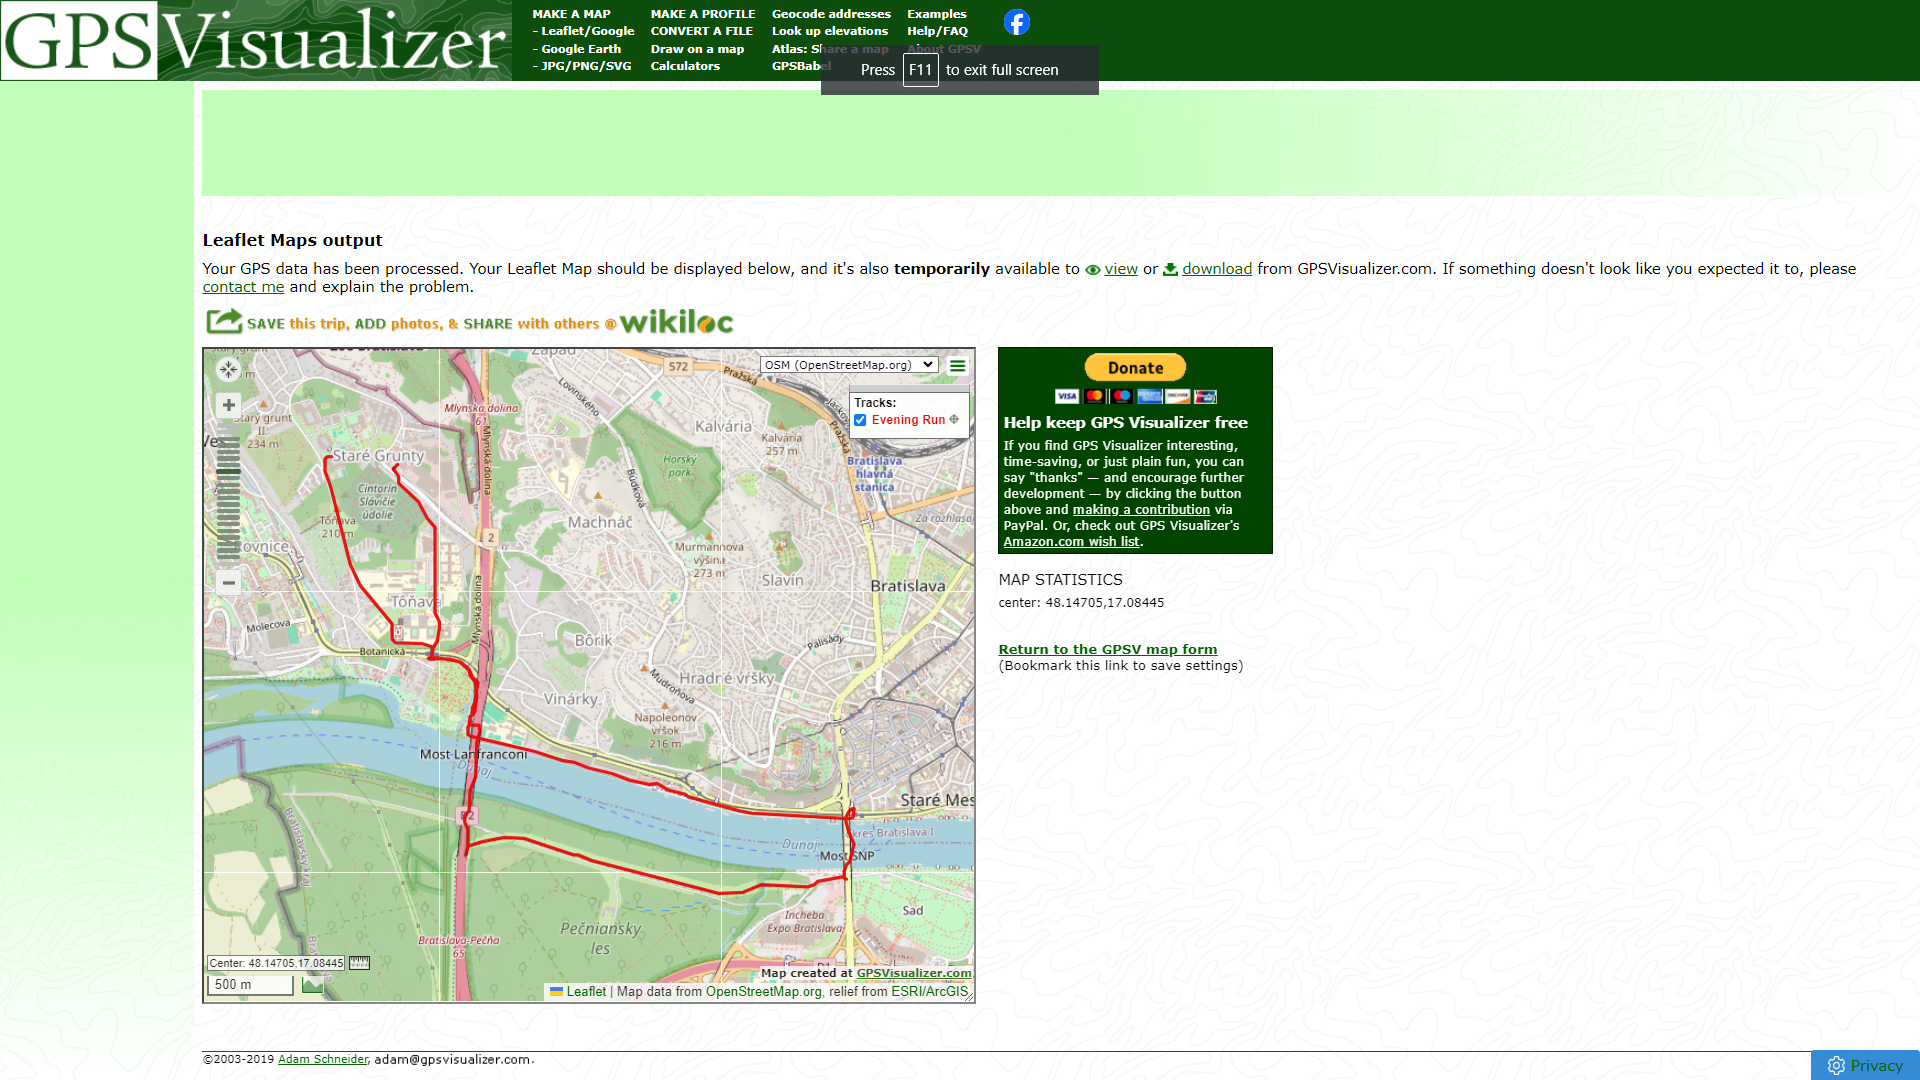
\includegraphics[width=1\textwidth]{img/gps_visualizer/gpsvisualizer2.png}
    \caption{Zobrazenie trasy}
  \end{subfigure}
  \caption{GPS Visualizer prostredie}
  \label{fig:gps-visualizer}
\end{figure}

\subsection{Moje riešenie}
Moje riešenie je webová aplikácia, pomocou ktorej si môže používateľ vizualizovať trasy na mape prehľadne. To znamená, že aj pri veľkom počte trás (10 a viac) prechádzajúcich tým istým miestom, môže používateľ nastaviť zobrazenie tak, aby bolo prehľadné a na mape nevznikali tzv. "špagety"(obr.\ref{fig:spagety}). Vďaka správnemu nastaveniu zobrazenia je možné vidieť trasy a cestnú sieť prehľadne. Používateľ sa môže v aplikácii registrovať a prihlásiť a teda je možné nahrané trasy zobraziť neskôr bez nutnosti znova trasy do aplikácie nahrať. Trasy sa do aplikácie nahrávajú v ZIP súbore, čo umožňuje nahrať viac trás súčasne. Tieto trasy je možné zobraziť na mape jednotlivo, alebo všetky naraz obsiahnuté v ZIP súbore. Aplikácia ponúka map-match funkcionalitu, čo znamená, že trasy budú pripnuté na cestnú sieť a tým sa zlepší viditeľnosť mapy a trás na mape, obrázok \ref{fig:niespagety}. 
\newline Výhody:
\begin{itemize}
  \item map-match, pripnutie trás na cestnú sieť pre zlepšenie viditeľnosti
  \item možnosť nahrať viac trás naraz
  \item zobrazenie vlastných trás po nahratí bez nutnosti nahrávať trasy pri každom zobrazení
  \item možnosť nahrať trasy vo viacerých formátoch (CSV,GEOJSON,GPX)
  \item neobmedzený počet zobrazení mapy s neobmedzeným počtom nahraných súborov (počet nahraných súborov je obmedzený veľkosťou vyhradeného miesta na serveri)
  \item do jednej požiadavky na map-match môže ísť až 20 tisíc súradníc
  \item informácia pre používateľa v prípade, že niektorá z trás nemala požadovaný formát 
\end{itemize}
Nevýhody:
\begin{itemize}
  \item jedna trasa môže obsahovať maximálne 20 tisíc bodov
  \item map-match pri pešej chôdzi nie úplný (viac v kapitole TODO)
  \item priebeh map-matchu ZIP súboru nie je zobrazený, iba jeho dokončenie
  \item aj pri nahratí jednej trasy je nutné vložiť trasu do ZIP súboru so špeciálne určenou štruktúrou (TODO zobraziť odkaz na štruktúru)
\end{itemize}
\begin{figure}[H]
  \centering
  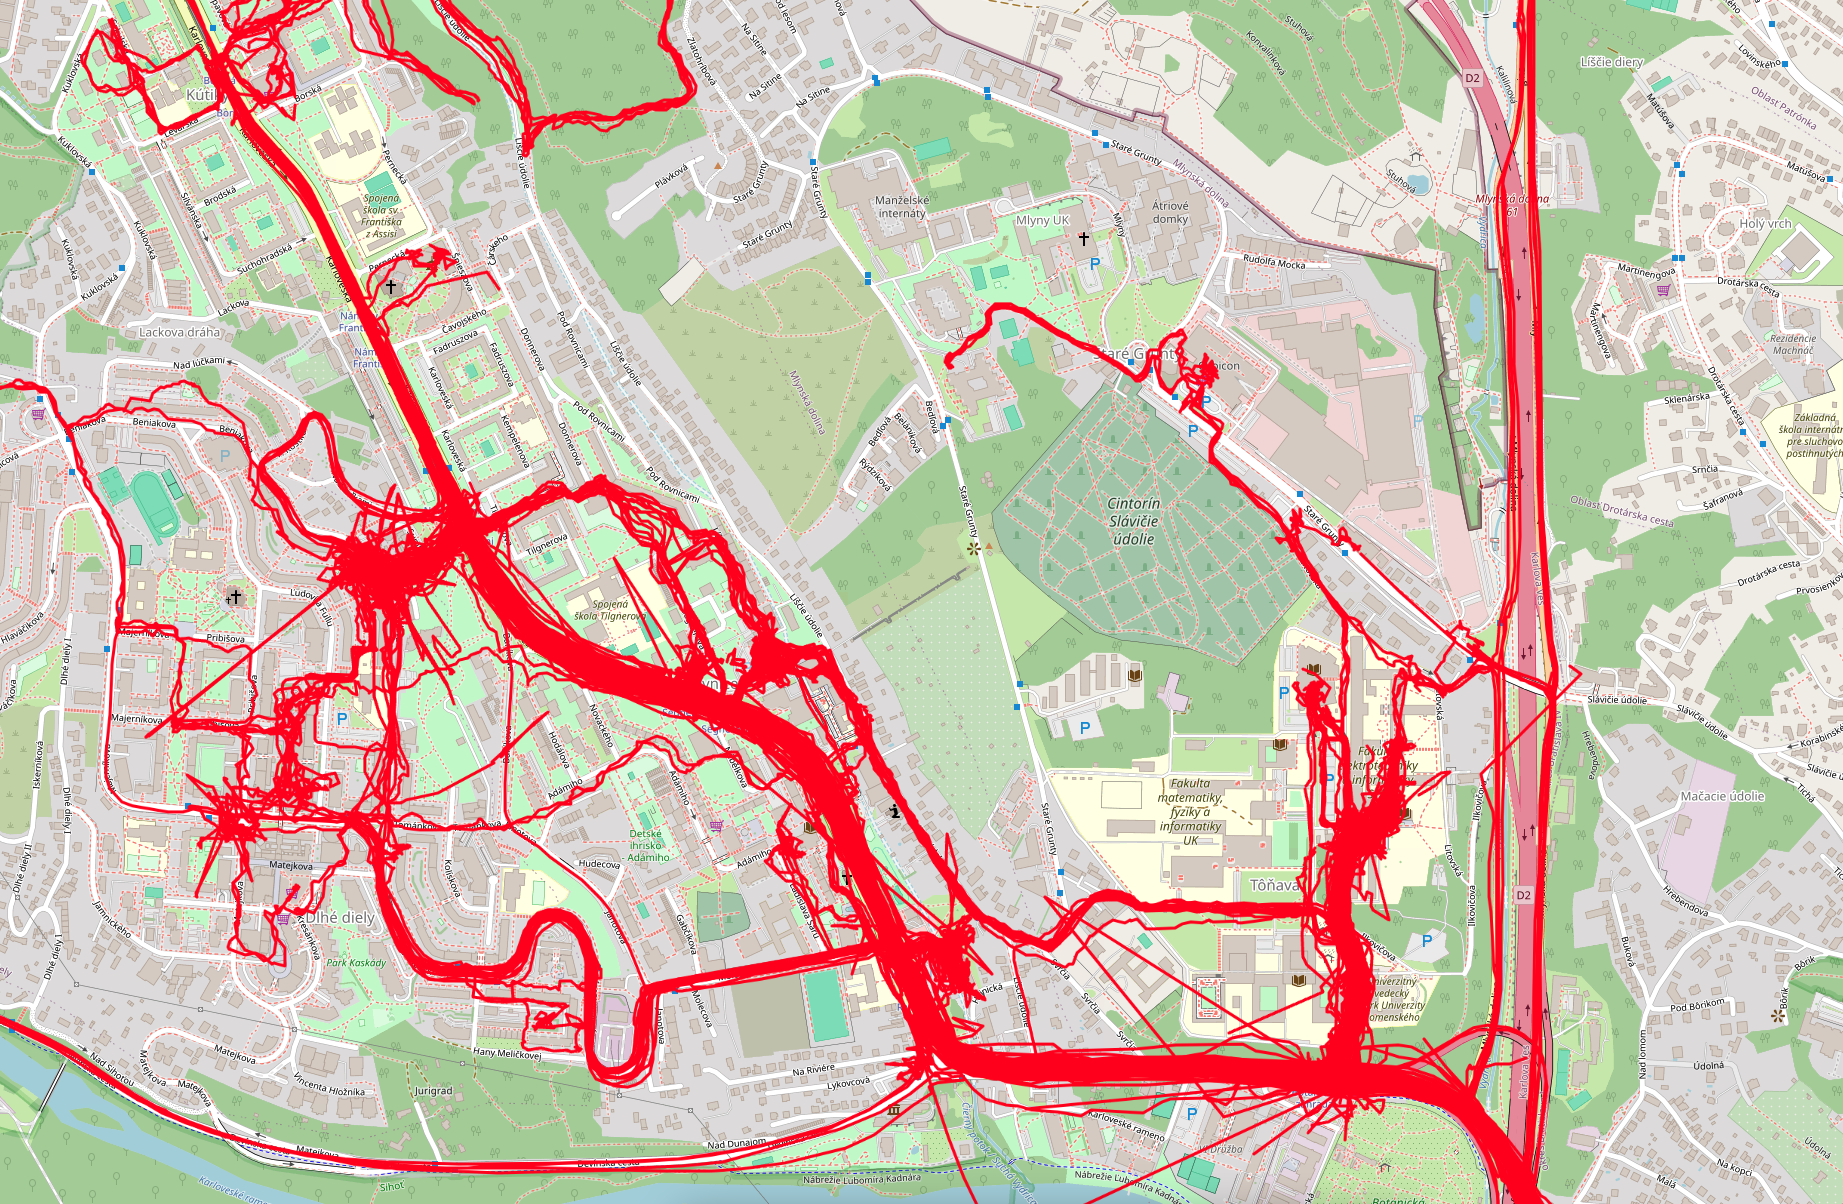
\includegraphics[width=0.7\textwidth]{img/map-match rozdiel/pred map-match.png}
  \caption{Zobrazenie väčšieho množstva trás na rovnakom mieste}
  \label{fig:spagety}
\end{figure}
\begin{figure}[H]
  \centering
  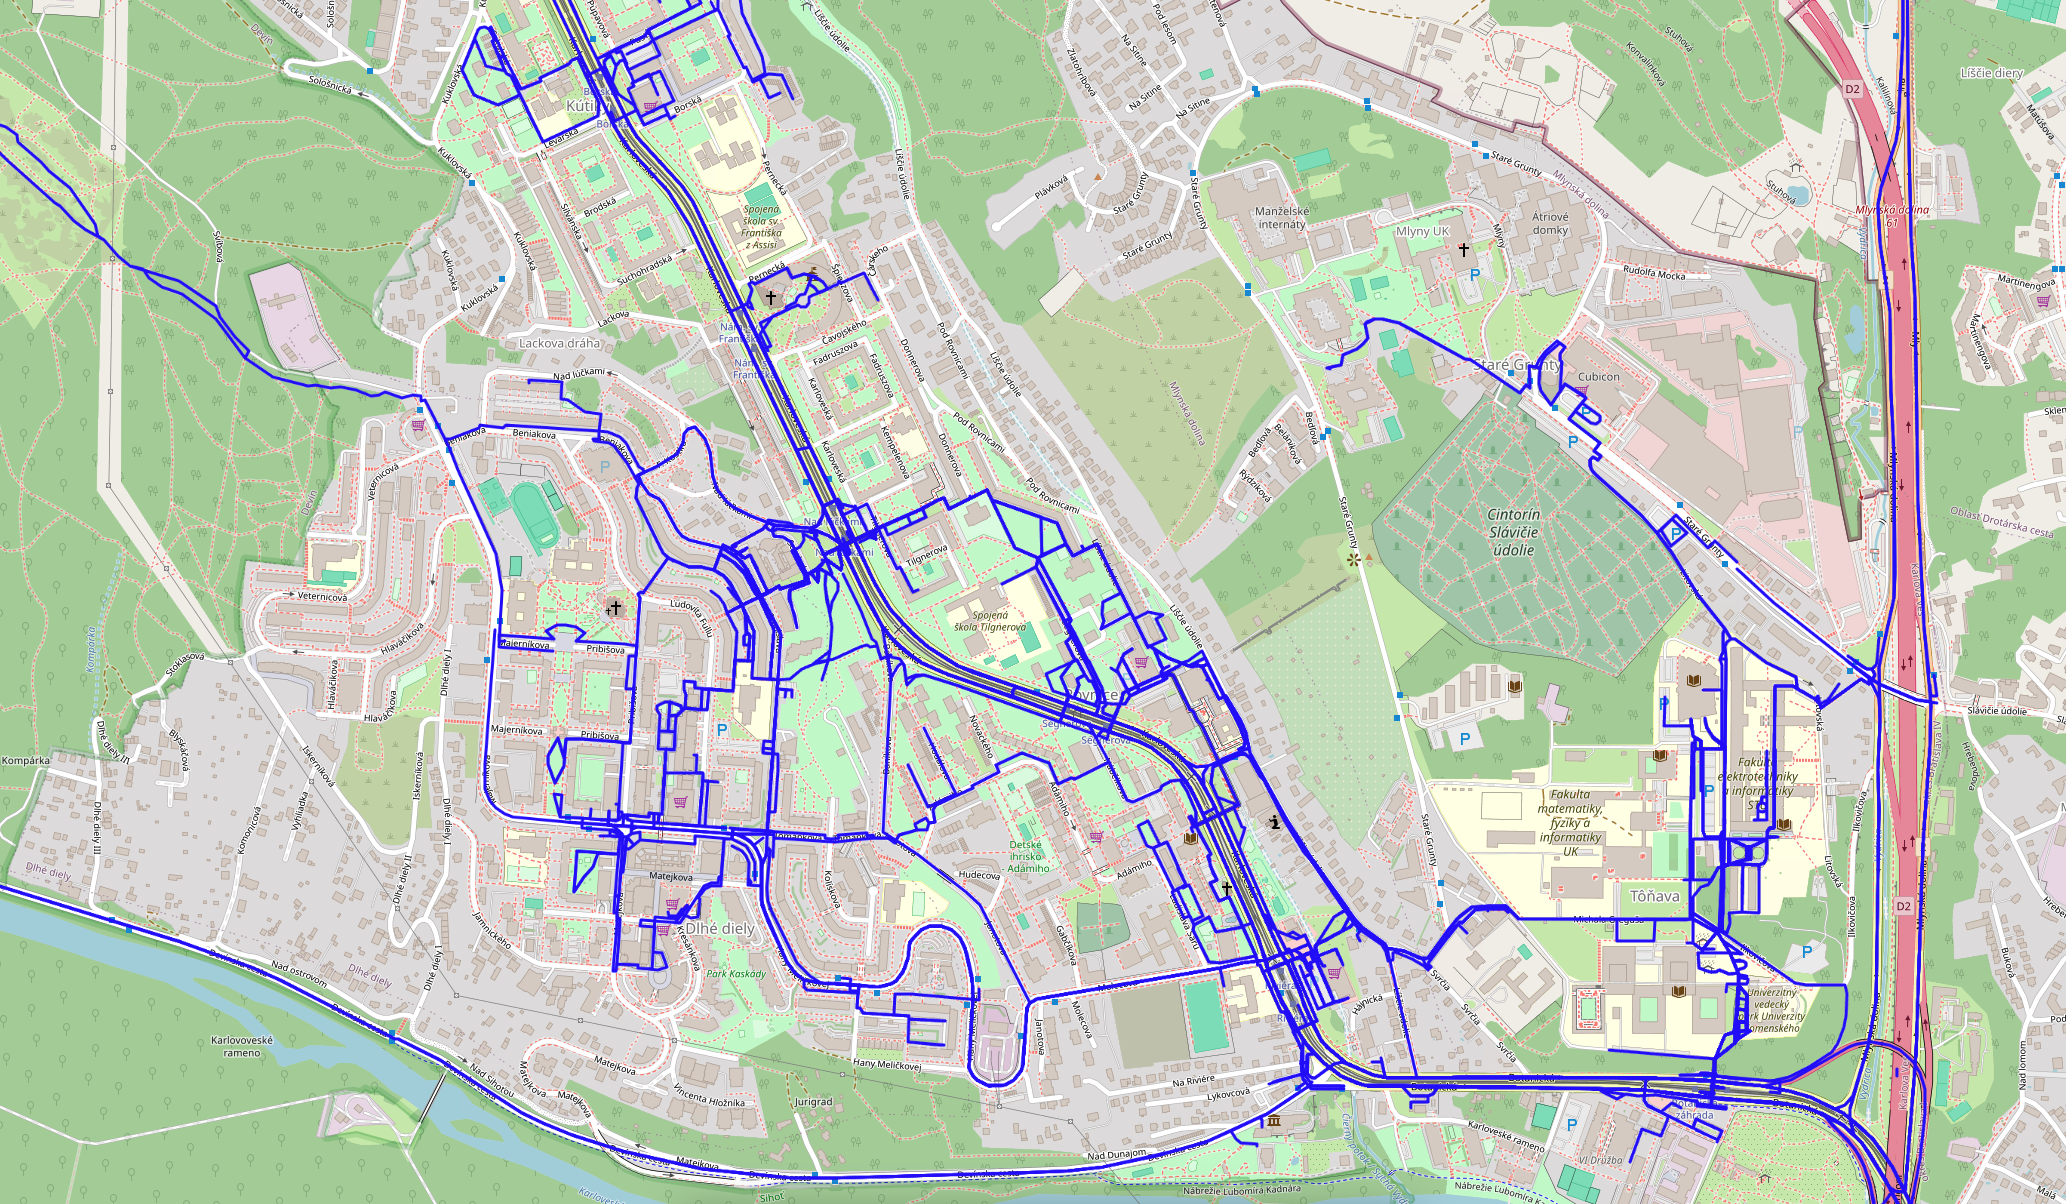
\includegraphics[width=0.7\textwidth]{img/map-match rozdiel/po map-match.png}
  \caption{Zobrazenie väčšieho množstva trás upravených map-matchom na rovnakom mieste}
  \label{fig:niespagety}
\end{figure}